\documentclass[../main.tex]{subfiles}

\begin{document}

\subsection{CXRS Diagnostics}
\subsubsection{CXRS for Plasma Measurements}

The Charge Exchange Recombination Spectroscopy (CXRS) diagnostics measures line emissions of several impurity isotopes in the plasma excited by charge exchange reactions with neutral hydrogen atoms injected into the plasma by the diagnostic neutral beam (DNB)~(\cref{eq:main_reaction_first,eq:main_reaction_second}). This line emission~(\cref{tab:cxrs_lines}) provides essential information for plasma control and physics studies: ion temperature $T_i$~(\cref{eq:ion_temperature}), toroidal ($v_\text{tor}$) and poloidal ($v_\text{pol}$) plasma rotation velocity~(\cref{eq:rotational_velocity}), helium ash and low Z impurity densities (beryllium, carbon, neon etc.) and the derived quantities such as $Z_\text{eff}$~(\cref{eq:impurity_density}).

\begin{align}
    X^{Z+} + H^0    & \to X^{(Z-1)+}(n_2) + H^+ \label{eq:main_reaction_first}   \\
    X^{(Z-1)+}(n_2) & \to X^{(Z-1)+}(n_1) + h\nu \label{eq:main_reaction_second}
\end{align}

% \begin{itemize}
%     \item Ion temperature $T_i$~--~line's width:
\begin{equation}
    \label{eq:ion_temperature}
    kT_\text{ion} = mc^2 \dfrac{{\Delta\lambda}_\text{Dopp}^2}{\lambda_{0}^{2}}
\end{equation}
where $k$~--~ Boltzmann constant, ${\Delta\lambda}_\text{dopp}$~--~line's width due to Doppler broadening, $\lambda_0$~--~\enquote{natural}, unshifted wavelength of the line's center.

% \item Rotation velocity $v_\text{rot}$~--~doppler shift of line's center:
\begin{equation}
    \label{eq:rotational_velocity}
    v_\text{rot} = c \dfrac{\Delta\lambda_\text{rot}}{\lambda_{0} \cos \alpha}
\end{equation}
where ${\Delta\lambda}_\text{rot}$~--~line's shift due to Doppler effect, $\alpha$~--~angle between line of sight and toroidal direction.

% \item Impurity's density $n_\text{imp}$ and $Z_\text{eff}$~--~intensity of the line:
\begin{equation}
    \label{eq:impurity_density}
    n_\text{imp} = \dfrac{4\pi \int I(\lambda)\, d\lambda}{n_\text{b} Q_\text{CX}^\text{eff}(v_\text{b})\, dl}
\end{equation}
where $I(\lambda)$~--~intensity of the line, $n_\text{b}$~--~local neutral beam density, $Q_\text{CX}^\text{eff}(v_\text{b})$~--~effective rate coefficient due to charge exchange, $l$~--~coordinate along a line of sight.
% \end{itemize}

\begin{table}[!ht]
    \caption{Spectroscopic lines used in CXRS.}%
    \label{tab:cxrs_lines}
    \centering
    \begin{tabular}[]{l l l}
        \toprule
        Ion       & Transition & Wavelength \\
        \midrule
        BeIV      & $6\to5$    & 465.8 nm   \\
        BeIV      & $8\to6$    & 468.5 nm   \\
        HeII      & $4\to3$    & 468.5 nm   \\
        \midrule
        ArXVIII   & $16\to15$  & 522.5 nm   \\
        NeX       & $11\to10$  & 524.9 nm   \\
        CVI       & $8\to7$    & 529.1 nm   \\
        \midrule
        H$\alpha$ &            & 656.3 nm   \\
        MSE       &            & 659.1 nm   \\
        \bottomrule
    \end{tabular}
\end{table}

\subsubsection{CXRS in ITER}
The CXRS Edge diagnostic is a distributed system with components throughout the ITER tokamak complex. The primary viewing components (front-end optics) are installed in Equatorial port 3 (EP3), viewing the Diagnostic Neutral Beam (DNB) that enters the plasma in the neighboring section 4.
Front-end optics consists of two light collecting systems: Upper and Lower. The scope of the 55.EC CXRS Edge diagnostic for Upper system ends at the image plane in the port interspace (11-L1-C03) where the collected signal is coupled into optical fibre bundles.
For Lower system, however, 55.EC CXRS Edge diagnostic is responsible for light collection system, light transportation and detection. The collected signal is transported through optical fibre bundles to the Tritium building (Building 14 – Level 2 – Room 4), where the detection systems are located.

\begin{figure}[htbp]
    \centering
    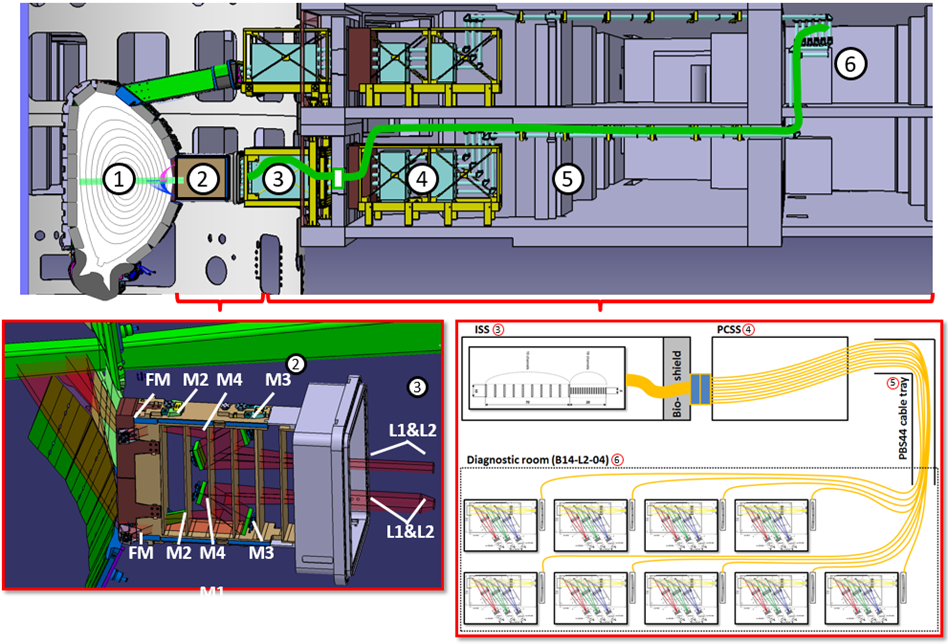
\includegraphics[width=0.75\textwidth]{images/cxrs_edge_overview}
    \caption{An overview of the CXRS Edge diagnostic design.}%
    \label{fig:cxrs_edge_overview}
\end{figure}

\subsection{Development of the New Simulation Code}
\subsubsection{Existing Code}
Simulation of Spectra (SOS) code by M. G. von Hellermann~\cite{sos}

Features:
\begin{itemize}
    \item Simulation takes into account many physical effects (halo effect, crossection effect, plume effect and others);
    \item Written in Matlab;
    \item Has Graphical User Interface~(\cref{fig:sos_interface}).
\end{itemize}

\begin{figure}[!ht]
    \centering
    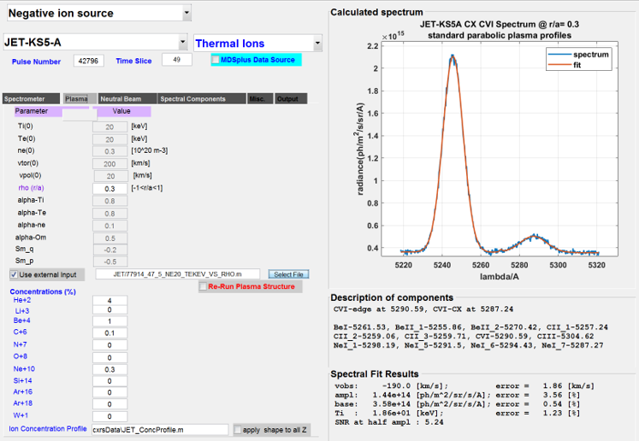
\includegraphics[width=0.75\textwidth]{images/sos_interface}
    \caption{SOS interface.}%
    \label{fig:sos_interface}
\end{figure}

\subsubsection{Motivation}
Existing code (Simulation of Spectra~--~SOS) lacks some features:
\begin{itemize}
    \item Simplified plasma, tokamak and diagnostic geometry \\
          (e.g. elliptical plasma, point emission and others);
    \item Does not take reflections into account;
    \item Cannot use data from IMAS directly;
    \item Requires Matlab license, hard to extend by new developers.
\end{itemize}

The goal was to create an open and extensible simulation code using Python.

Sub goals:
\begin{itemize}
    \item Implement interaction with IMAS database (read and write);
    \item Use IMAS data to create a plasma and diagnostic beam with spatial distributions;
    \item Use a ray-tracing engine to simulate spectra, this includes how reflections affect simulated spectra;
    \item Ensure that emission models include all physics already captured by SOS.
\end{itemize}


\subsection{Raysect and CHERAB}

\textbf{Raysect}~\cite{raysect} is a ray-tracing framework for Python designed for scientific purposes.
\begin{itemize}
    \item Supports scientific ray-tracing of spectra from physical light sources such as plasmas.
    \item Easily extensible, written with user customisation of materials and emissive sources in mind.
    \item Different observer types supported such as pinhole cameras and optical fibres.
\end{itemize}

\textbf{CHERAB}~\cite{cherab} is a Python library for forward modelling diagnostics based on spectroscopic plasma emission which provides physical models for Raysect.
Provided models for Raysect:
\begin{itemize}
    \item Tools for plasma and diagnostic beam simulations;
    \item Physical emission models (active charge exchange, bremsstrahlung and more).
\end{itemize}


\begin{figure}
    \centering
    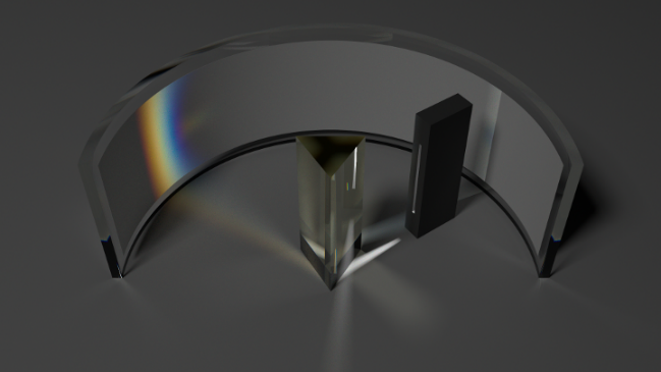
\includegraphics[width=0.75\textwidth]{images/raysect_demo}
    \caption{Demonstration of Raysect features.}%
    \label{fig:raysect_demo}
\end{figure}

\end{document}